\documentclass[]{article}

\usepackage[T1]{fontenc}
\usepackage{graphicx}
\title{\textbf{\huge Werkzeuge für das wissenschaftliche Arbeiten}\\
	Python for Machine Learning and Data Science\\}
\usepackage[ngerman]{babel}
\usepackage[utf8]{inputenc}


\begin{document}
\maketitle
{ \centerline\small\hspace*{4.5cm}Abgabe: 9.12.2022} \\

\hrulefill
\tableofcontents %Inhaltsverzeichnis
\hrulefill

\section{Projektaufgabe}
In dieser Aufgabe beschäftigen wir uns mit Objektorientierung in Python.
Der Fokus liegt auf der Implementierung einer Klasse, dabei nutzen wir insbesondere auch Magic Methods.\\
\begin{figure}[htbp]
\begin{minipage}{\linewidth}
\renewcommand{\footnoterule}{}
\begin{center}
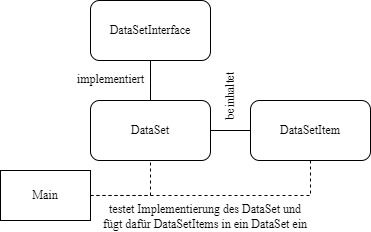
\includegraphics[width=0.7\linewidth]{./../diagram/classes_files.jpg}.
\end{center}
\caption[Darstellung der Klassenbeziehungen.]{Darstellung der Klassenbeziehungen.}
\end{minipage}
\end{figure}
\subsection{Einleitung}
Ein Datensatz besteht aus mehreren Daten, ein einzelnes Datum wird durch ein Objekt der Klasse \grqq DataSetItem\grqq{} repräsentiert.
Jedes Datum hat einen Namen (Zeichenkette), eine ID (Zahl) und bel. Inhalt.\\
\\
Nun sollen mehrere Daten, Objekte vom Typ \grqq DataSetItem\grqq{}, in einem Datensatz zusammengefasst werden.
Sie haben sich schon auf eine Schnittstelle und die benötigen Operationen, die ein Datensatz unterstützen muss, geeinigt.
Es gibt eine Klasse \grqq DataSetInterface\grqq{}, die die Schnittstelle definiert und Operationen jedes Datensatzes angibt.
Bisher fehlt aber noch die Implementierung eines Datensatzes mit allen Operationen.\\
\\
Implementieren Sie eine Klasse \grqq DataSet\grqq{} als eine Unterklasse von \grqq DataSetInterface\grqq .\\
\\
\subsection{Aufbau}
Es gibt drei Dateien, \grqq dataset.py\grqq, \grqq main.py\grqq{}  und \grqq implementation.py\grqq \footnote{Dateien befinden sich im Ordner \grqq /code/\grqq{} dieses Git-Repositories.}.
In der \grqq dataset.py\grqq{} befinden sich die Klassen \grqq DataSetInterface\grqq{} und \grqq DataSetItem\grqq ,
in der Datei \grqq implementation.py\grqq{} muss die Klasse \grqq DataSet\grqq{} implementiert werden.
Die Datei \grqq main.py\grqq{} nutzt die Klassen \grqq DataSet\ \grqq{} und \grqq DataSetItem\ \grqq{} aus den jeweiligen Dateien und testet die Schnittstelle und Operationen von \grqq DataSetInterface\grqq .\\
\\
\subsection{Methoden}
Bei der Klasse \grqq DataSet\grqq{} sind insbesondere folgenden Methoden zu implementieren, die genaue Spezifikation finden Sie in der \grqq dataset.py\grqq :\\
\begin{itemize}
    \item \_\_setitem\_\_(self, name, id\_content)\\
\hspace*{1cm} Hinzufügen eines Datums, mit Name, ID und Inhalt
\item \_\_iadd\_\_(self, item)\\
\hspace*{1cm} Hinzufügen eines \grqq DataSetItem\grqq
\item\_\_delitem\_\_(self, name)\\
\hspace*{1cm}Löschen eines Datums auf Basis des Namens.
Das heißt auch, dass der Name eines Datums ein eindeutiger Schlüssel ist und jeder Name nur einmal pro Datensatz vorkommen kann.
\item \_\_contains\_\_(self, name)\\
\hspace*{1cm} Prüfung, ob ein Datum mit diesem Namen im Datensatz vorhanden ist.
\item \_\_getitem\_\_(self, name)\\
\hspace*{1cm} Abrufen des Datums über seinen Namen.
\item \_\_and\_\_(self, dataset)\\
\hspace*{1cm} Schnittmenge zweier Datensätze bestimmen und als einen neuen Datensatz zurückgeben.
\item \_\_or\_\_(self, dataset)\\
\hspace*{1cm} Vereinigungen zweier Datensätze bestimmen und als einen neuen Datensatz zurückgeben.
\item \_\_iter\_\_(self)\\
\hspace*{1cm} Iteration über alle Daten den Datensatzes (es ist möglich eine Sortierung für die Reihenfolge der Iteration anzugeben).
\item filtered\_iterate(self, filter)\\
\hspace*{1cm} Gefilterte Iteration über einen Datensatz, dabei dient eine Lambda-Funktion mit den Parametern Name und ID für jedes Datum als Filter.
\item \_\_len\_\_(self)\\
\hspace*{1cm} Anzahl der Daten in einem Datensatz abrufen.

\end{itemize}

\section{Abgabe}
Programmieren Sie die Klasse \grqq DataSet\grqq{} in der Datei \grqq implementation.py\grqq{} zur Lösung der oben beschrieben Aufgabe im VPL.
Sie können auch direkt auf Ihrem Computer programmieren, dazu finden Sie alle drei benötigten Dateien zum Download im Moodle.\\
\\
Das VPL nutzt den gleichen Code, wobei die \grqq main.py\grqq{} um weitere Testfälle und Überprüfungen erweitert wurde.
Die Überprüfungen dienen dazu sicherzustellen, dass Sie die richtigen Klassen nutzen.\\
\end{document}